In this section we introduce the general architecture of a game. We then present an example of common timing and synchronization primitives used in DSL's for games and we show some techniques typically used to implement them. For each technique we list the main drawbacks. Finally we present our solution to the problem of developing a DSL for games.

\subsection{Preliminaries}
A game engine is usually made by several interoperating components. All the components use a shared data structure, called \textit{game state}, for their execution. The two main components of a game are the \textit{logic engine}, which defines how the game state evolves during the game execution, and the \textit{graphics enginge}, which draws the scene by reading the updated game state. These two components are executed in lockstep within a function called \textit{game loop}. The game loop is executed indefinitely, updating the game state by calling the logic engine, and drawing the scene by using the graphics engine. An iteration of the game loop is called \textit{frame}. Usually a game should run between 30 to 60 frames per second. This requires both the graphics engine and the logic engine to be high-performance. In this paper we will only take into account the performance of the logic engine, as scripting drives the logic of the game loop. A schematic representation of this architecture can be seen in Figure \ref{fig:game_loop}.

\begin{figure}
	\centering
	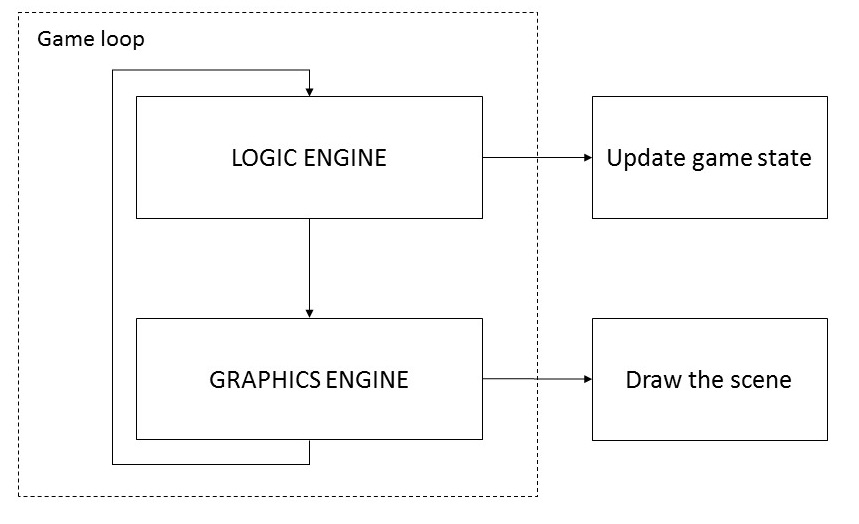
\includegraphics[scale=0.3]{Pictures/game_loop}
	\caption{Game loop}
	\label{fig:game_loop}
\end{figure}

\subsection{A time and synchronization primitive}
\label{subsec:synchronization}
A common requirement in game DSL's is a statement which allows to pause the execution of a function for a specified amount of time or until a condition is met. We will refer to these statements as \texttt{wait} and \texttt{when}. Such a behaviour can be modelled using different techniques:

\begin{itemize}
	\item \textit{Threads} allow to solve such synchronization problems but they are unsuitable for video game development because of memory usage and CPU overhead due to their scheduling.
	\item \textit{Finite State Machines} allow to represent such concurrent behaviours \cite{CASANOVA2_PAPER} by using a \texttt{switch} control structure to an opportune state. For instance in the case of timed wait, the states are \textit{wating} and \texttt{clear} (when the timer has elapsed). This solution is high-performance but the logic of the behaviour is lost inside the \texttt{switch} structure.
	\item \textit{Strategy pattern} allows to represent the instructions of the language has polymorphic data types. Each concurrent structure is implemented by a class which defines the behaviour of the current structure, and the next structure to execute. This solution is not high-performance due to virtuality and the high number of object instantiations.
	\item \textit{Monadic DSL} uses a variation of the state monad. It represents scripts with two states: \textit{Done} and \textit{Next}. The bind operator is used to simulate the code interruption. This approach is simple and elegant but it suffers of the same virtuality problems of the strategy pattern, this time because of the extensive use of lambda expressions.
	\item \textit{Compiled DSL} is the most common solution and allows to represent the concurrency by using concurrent control structures defined in the language. Compiled DSL's grant high-performance and code readability, but they require to implement a compiler or an interpreter for it.
\end{itemize}

In what follows we show a possible implementation of these statements using the presented techniques. We deliberately ignore the thread-based implementation since, as explained above, threads are not suitable for game development.

\paragraph{Monadic DSL:} A possible approach to building an interpreted DSL is using monads in a functional programming language, as done in \cite{CASANOVA1_PAPER}. A script is a function that takes no input parameters and returns the state of the script after the execution of the current statement. The state can be either \textit{Done}, when the script terminates, or \textit{Next} when the script is still running and we need to pass the rest of the script to be evaluated. We present a definition of the monad in the following code snippet in pseudo-ml:

\begin{lstlisting}
type Script<'a> = Unit -> State<'a>
and State<'a> = Done of 'a | Next of Script<'a>
\end{lstlisting}

\noindent
We can define the \texttt{Return} and \texttt{Bind} operators as follow:

\begin{lstlisting}
let return (x : 'a) : Script<'a> =
  fun () -> Done x
  
let (p : Script<'a>) >>= (k : 'a -> Script<'b>) : Script<'b> =
  fun () ->
    match p with
    | Done x -> k x ()
    | Next p' -> Next(p' >>= k)
\end{lstlisting}

\noindent
The \texttt{Return} operator simply returns a script that builds the result of the computation. The \texttt{Bind} operator checks the current state of the script: if the script has terminated then it simply builds the result by executing the last script statement, otherwise it returns the continuation containing the invocation of the \texttt{Bind} on the remaining part of the script. In this framework the \texttt{wait} statement can be implemented as follows (we assume that \texttt{do} is a shortcut for the bind on a function returning \texttt{Script<Unit>}):

\begin{lstlisting}
let yield : Script<Unit> =
  fun () -> Next(fun () -> Done ())

let rec waitRecursion (interval : float32, 
                       startingTime : float32) : Script<Unit> =
  let t = getTime()
  let dt = (t - t0)
  if dt < interval then
    do yield
    do waitRecursion(startingTime)
  else
    return ()
      
let wait (timer : float32) : Script<Unit> =
  let t0 = getTime()
  do waitRecursion(timer, t0)
  
let when (predicate : Unit -> bool) : Script<Unit> =
  if predicate () then return ()
  else
    do yield
    do when predicate
\end{lstlisting}
\noindent
The \texttt{yield} function simply forces the script to stop for one frame. The \texttt{wait} function recursively checks if the timer has elapsed. If this is not the case it skips a frame and then re-evaluates otherwise it returns \texttt{Unit}. \texttt{wait} on a predicate simply skips a frame and keeps re-executing itself until the condition is met.

\paragraph{Strategy pattern} Implementing \texttt{wait} and \texttt{when} with the strategy pattern requires to define an interface which contains the signature for a method to run the script. Usually scripts need to access the time elapsed between the current frame and the previous one and to a reference to the game state data structure for various reasons, which are passed as parameter for this method. The method returns the updated script after the current execution. We present the code for the interface in a pseudo-C\# code:

\begin{lstlisting}
public interface Script
  public Script Run(float dt, GameState state);
\end{lstlisting}

We will then model \texttt{wait} and \texttt{when} with two classes implementing such interface. Each of the script commands contains a reference to the next statement to execute.

\begin{lstlisting}
public class Wait : Statement
  private Statement next;
  private float time;
  
  public Script Run(float dt, GameState state)
    if (time >= 0)
      time -= dt;
      return this;
    else
      return next;

public class When : Statement
  private Func<bool> predicate;
  private Script next;
  
  public Script Run(float dt, GameState state)
    if (predicate())
      return next;
    else
      return this;
\end{lstlisting}

\paragraph{Finite state machines:} In this approach we model \texttt{wait} and \texttt{when} as finite state automata. Both statements require to store the state of the automata. \texttt{wait} requires to store a timer whose value is updated at each frame. \texttt{when} stores a predicate to execute and check at every game logic update. \texttt{wait} has three states: (\textit{i}) timer initialization, (\textit{ii}) check timer and update, and (\textit{iii}) timer elapsed. In the first state we initialize the timer and then update it for the first time. The second state is used to check whether the timer has elapsed. The third state is used to continue with the execution after the time has elapsed.

\begin{lstlisting}
//WAIT
public void Update(float dt, GameState gameState)
  switch(state)
    case -1: 
      this.t = timer;
      state = 0;
      goto case 0;
    case 0:
      this.t = this.t - dt
      if (this.t <= 0)
        state = 1;
        goto case 1:
      else
        return;
    case 1:
    //run the code after wait
\end{lstlisting}

\texttt{when} has two states: (\textit{i}) check predicate, (\textit{ii}) predicate satisfied (go on with the execution). The first state checks if the predicate has been satisfied. If that is the case, we jump to the next state, otherwise we pause the execution and we remain in the same state.

\begin{lstlisting}
//WHEN
public void Update(float dt, GameState gameState)
  switch(state)
    case 0:
      if (predicate())
        state = 1;
        goto case 1:
      else
        return;
    case 1:
    //run the code after when
\end{lstlisting}

\paragraph{Waiting with a hard-coded compiler:} This approach requires to build a compiler by generating the syntax using a standard lexer/parser generator. After that usually it is required to define a set of type rules, and the operational semantics of the language constructs. The type rules and the operational semantics are then implemented in the type checker and the code generator of the compiler.

\subsection{Discussion}
In the previous paragraph we have seen different techniques employed by developers to implement timing and synchronization statements commonly used in video games. We now list the advantages and disadvantages of each solution:

\begin{itemize}
	\item \textit{Monadic DSL:} this solution is elegant but inefficient, because of the extensive use of lambda expressions in monads. Indeed lambdas are usually implemented with virtual method calls. The code to define a monadic DSL is compact.
	\item \textit{Strategy Pattern:} this solution is simple but low-performance because of the virtual method calls the logic update must invoke to run the statements and the high number of object instantiation to generate the script statements (one per statement). Besides the readability of the program for long scripts is lost due to the long chain of object instantiations. A library supporting scripts implemented with the strategy pattern is compact.
	\item \textit{Finite state machines:} this approach is high-performance due to the small overhead of the \texttt{switch} control structure. Unfortunately the logic of the program for very complex scripts with several nested synchronizations is lost inside huge \texttt{switch} structures and the complexity increases drastically with the number of interruptions and synchronizations in the script \cite{AI_GAMES}. Moreover note that for each timer we have to maintain a separate timer, and for any of the two control structures we need to store the state of the automaton. Implementing complex synchronizations require long and complex state machines.
	\item \textit{Hard-coded compiler:} this approach is high-performance, as we could generate the state machines presented above during the code generation step, but building, maintaining, and extending a hard-coded compiler is a hard and time-consuming task. The code length increases with the size of the compiler (in term of modules and code lines) and the language complexity.
\end{itemize}
This situation is summarized in Table \ref{tab:techniques}.

\begin{table}
	\small
	\centering
	\begin{tabular}{|c|c|c|c|}
		\hline
		Technique & Readability & Performance & Code length \\
		\hline
		Monadic DSL & \checkmark & \ding{55} & \checkmark \\
		\hline
		Strategy Pattern & \ding{55} & \ding{55} & \checkmark \\
		\hline
		Finite state machines & \ding{55} & \checkmark & \ding{55} \\
		\hline
		Hard-coded compiler & \checkmark & \checkmark & \ding{55} \\
		\hline
	\end{tabular}
	\caption{Pros and cons of script implementation techniques}
	\label{tab:techniques}
\end{table}

In this work we propose another development approach in building a game DSL by using a metacompiler, a program which takes as input a language definition, a program written in that language, and generates executable code.

\noindent
Given this considerations, we formulate the following problem statement.

\vspace{0.5cm}
\noindent
\textbf{PROBLEM STATEMENT:}
Given the formal definition of a game DSL our goal is to automate, by using a metacompiler, the process of building a compiler for that language in a (\textit{i}) short (code lines), (\textit{ii}) clear (code readability), and (\textit{iii}) efficient (time execution) way, with respect to a hand-made implementation.